\chapter{Evaluation}
\label{eval}

In this chapter, we first present an example of SMEIL used as an \gls{il}
followed by four small examples implemented in SMEIL: A model watch using a
7-segment display, the core of a trading chip, a process for binning colors
based on intensity and finally a MD5 hash bruteforcer.  \todo{Motivate why
  these examples were picked in particular}

Information on how to reproduce the runs shown below is given in \Cref{app:inst}.


\section{SMEIL as an intermediate language}
\label{sec:smeilil}
We have made repeated references to the origins of SMEIL as a pure \gls{il} and
described how and why the scope of the language was expanded to also include the
use as an independent implementation language. Despite this, SMEIL is still very
much intended to be also usable as an \gls{il}. As it may be obvious at this
point, the design, implementation and testing have mostly focused on its use as
a primary implementation language, with the \gls{il} angle remaining in the
background. Ideally, we would have developed a code generation backend for C\#
at this point, targeting SMEIL, since that is the most complete SME
implementation. %Unfortunately?
However, this was not possible within the available time-frame
and in any case, the implementation would need to be carried out by a third
party, and this was outside the scope of the thesis.
% --- your present writer is not sufficiently familiar with the C\# SME framework
% to carry out the work himself within a reasonable time frame. In the end, time
% had to be prioritized and the time required to show a functioning and automated
% proof-of-concept using SMEIL as an intermediate language would have sacrificed
% significant parts of the co-simulation interface.

%It is never ideal to leave loose ends, so
To show that using SMEIL as an \gls{il} {\itshape can} be done, we have adapted
our previously implemented Python to \gls{vhdl} compiler to generate SMEIL
instead of generating VHDL directly. This translation is not yet fully
automated, but we explain how that could be done feasibly.

As an example, we will show how the SomeOps network is translated from PySME to
SMEIL.  This implementation was first presented in~\cite{asheim2016vhdl} and is
shown here with very minor modifications. The network, shown in
\Cref{fig:someops}, is configured as follows: A generator process continuously
emits two numbers through a shared bus.  Two processes are connected to the
reading end of the bus which will add and multiply the numbers,
respectively. The results of the calculation is then printed by the Printer
process.  The PySME code of the network is shown in \Cref{fig:someopspy}. The
code uses a slightly older version of the PySME library than used elsewhere in
this thesis which has some minor differences, for example, the {\ttfamily
  self.tell} function which was renamed to {\ttfamily self.add}.  SME processes
are declared using a class extending one of the classes {\ttfamily External} or
{\ttfamily Function}.  The two classes are semantically identical, but are used
to indicate if a process is intended purely for simulation or for hardware
synthesis, respectively.  Thus, {\ttfamily External} processes are expected to
utilize code constructs not representable on hardware.  The translator handled
these constructs by simply generating empty entity declarations in their place.

The generated SMEIL code is shown in \Cref{fig:someopssme} with a manually added
{\tt trace} statement to the {\tt Printer} process for printing the calculation
result. We can observe that it is possible to transform the PySME program to SMEIL
in a straightforward manner. Different from most of the other SMEIL examples
shown elsewhere, this code utilize a different strategy for creating connections
between processes where both input and output buses are explicitly passed as
parameters to the processes. This is the only possible way of connecting
processes in PySME (as described in \Cref{sec:sme2}). Thus, our idea of
providing a high-degree of flexibility in how network connections are created
(discussed in \Cref{sec:instance}) allows this PySME example to be translated
without any structural transformations.

For this process to be automated all that is needed is
\begin{itemize}
  \item Instead of converting {\ttfamily External} processes to empty processes
    in SMEIL, they should be omitted from the generated code.
  \item The PySME library should be able to replace buses going between
    {\ttfamily External} and {\ttfamily Function} processes in the Python
    program with connections to the {\ttfamily exposed} buses of the generated
    SMEIL code.
\end{itemize}
With these two changes in place, PySME programs will be able to use SMEIL as an
intermediate target for generating VHDL and to create test-files through the
co-simulation interface.

% The example is a shortened version of an example named AllOps which additionally
% performed division and multiplication.
% Since this code uses a slightly older
% version of the PySME library, we will briefly describe the differences between
% the PySME code used in this example and the PySME code appearing elsewhere in
% the thesis.


\begin{figure}
  \centering
  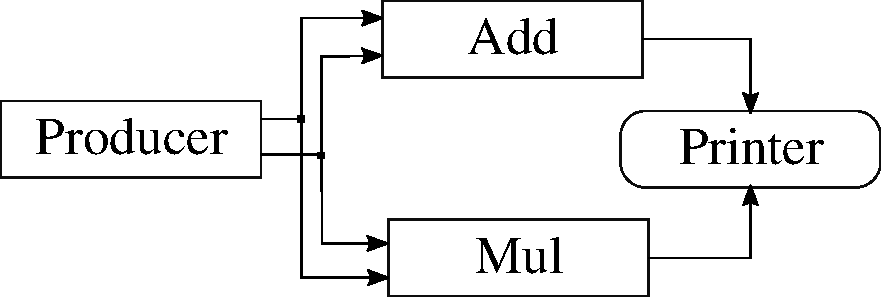
\includegraphics[width=0.6\textwidth]{figures/someopsnet.pdf}
  \caption{Schematics of the SomeOps network. Figure from \cite{asheim2016vhdl}.}
  \label{fig:someops}
\end{figure}

\begin{widefigure}
  \begin{subfigure}[t]{0.49\textwidth}
  \begin{pythoncode}
from sme import *
t = Types()

class Producer(Function):
  def setup(self, ins, outs):
    self.map_outs(outs, "outp")
    self.v1 = 0  # type: t.u7
    self.v2 = 0  # type: t.u7

  def run(self):
    self.outp["val1"] = self.v1
    self.outp["val2"] = self.v2
    self.v1 += 1
    self.v2 += 1
    if self.v1 > 100:
      self.v1 = 0
      self.v2 = 0

class Add(Function):
  def setup(self, ins, outs):
    self.map_ins(ins, "valbus")
    self.map_outs(outs, "addbus")

  def run(self):
  self.addbus["res"] = self.valbus["val1"] +
             self.valbus["val2"]

class Mul(Function): # Snipped (similar to Add)

class Printer(External):
  def setup(self, ins, outs):
    self.map_ins(ins, "addbus", "mulbus")

  def run(self):
    print(self.addbus["res"],
          self.mulbus["res"])

class SomeOps(Network):
  def wire(self):
    valbus = Bus("ValueBus", [t.u7("val1"),
                              t.u7("val2")])
    valbus["val1"] = 0
    valbus["val2"] = 0
    addbus = Bus("AddBus", [t.u8("res")])
    addbus["res"] = 0
    mulbus = Bus("MulBus", [t.u14("res")])
    mulbus["res"] = 0
    prod = Producer("Producer", [], [valbus])
    add = Add("Add", [valbus], [addbus])
    mul = Mul("Mul", [valbus], [mulbus])
    printer = Printer("Printer",
                      [addbus, mulbus], [])
    self.tell(printer) # 6x self.tell snipped
# Main function snipped
\end{pythoncode}
\caption{Original Python SME code.}
\label{fig:someopspy}
\end{subfigure}
\begin{subfigure}[t]{0.49\textwidth}
  \begin{smeilcode}
sync proc Add (in valbus, out addbus)
{
    addbus.res = valbus.val1 + valbus.val2;
}

sync proc Mul (in valbus, out mulbus)
{
    mulbus.res = valbus.val1 * valbus.val2;
}

sync proc Printer (in addbus, in mulbus)
{
    // Manually added
    trace("Add result: {} Mul result: {}",
        addbus.res, mulbus.res);
}

sync proc Producer (out outp)
    var v2: u7 = 0;
    var v1: u7 = 0;
{
    outp.val1 = v1;
    outp.val2 = v2;
    v1 = v1 + 1;
    v2 = v2 + 1;
    if (v1 > 100) {
        v1 = 0;
        v2 = 0;
    }
}

network SomeOps ()
{
    exposed bus AddBus {res: u8;};
    exposed bus MulBus {res: u14;};
    exposed bus ValueBus {val1: u7;
                          val2: u7;};
    instance Add of Add(ValueBus, AddBus);
    instance Mul of Mul(ValueBus, MulBus);
    instance Printer of Printer(AddBus, MulBus);
    instance Producer of Producer(ValueBus);
}

\end{smeilcode}
\caption{Generated SMEIL code.}
\label{fig:someopssme}
\end{subfigure}
\caption{Example of PySME code automatically translated to SMEIL.}
\end{widefigure}


\section{7-Segment Display}
\label{sec:7seg}
\begin{figure}%[tb]
\begin{minipage}{\linewidth}
  \centering
  \resizebox{.6\linewidth}{!}{
    \begin{tikzpicture}[font=\small,
      rep style/.style={rectangle,draw=black,text width=1.5cm,minimum
        size=1.5cm,align=center},
      proc style/.style={ellipse,draw=black,align=center,text
        width=1.5cm,minimum size=1.5cm,align=center},
      file style/.style={ellipse,draw=none,align=center,text
        width=1.5cm,minimum size=0.5cm,align=center},
      part/.pic={
        \node[] (m1) {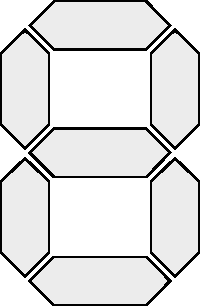
\includegraphics[width=.10\textwidth]{figures/7seg.pdf}};
        \node[left=0cm of m1] (m2) {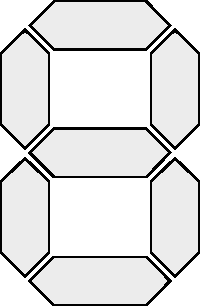
\includegraphics[width=.10\textwidth]{figures/7seg.pdf}};}
      ]

      \pic[local bounding box=hrs] {part};
      \node[below=2mm of hrs] (h2) {Hours};
      \pic[local bounding box=mins, right=30mm of hrs] {part};
      \node[below=2mm of mins] (m2) {Minutes};
      \pic[local bounding box=secs, right=30mm of mins] {part};
      \node[below=2mm of secs] (s2) {Seconds};

      \node[proc style, above=0.3cm of hrs] (dechrs) {Decoder};
      \node[proc style, above=0.3cm of mins] (decmins) {Decoder};
      \node[proc style, above=0.3cm of secs] (decsecs) {Decoder};

      \node[proc style, above=1cm of dechrs] (enchrs) {Encoder};
      \node[proc style, above=1cm of decmins] (encmins) {Encoder};
      \node[proc style, above=1cm of decsecs] (encsecs) {Encoder};
      
      \node[proc style, above=1cm of enchrs] (splithrs) {Calculate\\Hours};
      \node[proc style, above=1cm of encmins] (splitmins) {Calculate\\Minutes};
      \node[proc style, above=1cm of encsecs] (splitsecs) {Calculate\\Seconds};

      \draw[-{Latex[scale=1.6]}] (splithrs) edge (enchrs);
      \draw[-{Latex[scale=1.6]}] (splitmins) edge (encmins);
      \draw[-{Latex[scale=1.6]}] (splitsecs) edge (encsecs);

      \node[above=1cm of splitmins] (split) {};
      
      \node[proc style, above=2.5cm of split] (gen) {Timer};
      \draw[-] (gen) edge node [below left=0cm and 0cm of
      gen] {Seconds today} (split);

      \draw[-{Latex[scale=1.6]}] (split) edge (splithrs);
      \draw[-{Latex[scale=1.6]}] (split) edge (splitmins);
      \draw[-{Latex[scale=1.6]}] (split) edge (splitsecs);

      \draw[-{Latex[scale=1.6]}] (enchrs) edge (dechrs);
      \draw[-{Latex[scale=1.6]}] (encmins) edge (decmins);
      \draw[-{Latex[scale=1.6]}] (encsecs) edge (decsecs);

      \begin{scope}[on background layer]
        \node[draw=gray,inner sep=8pt,rounded corners=10pt,anchor=north
        west,fit=(enchrs)(encmins)(encsecs)(splithrs)(splitmins)(splitsecs)(gen),
        label={above}:Controller]
        (showhrs) {};
        \node[draw=gray,inner sep=8pt,rounded
        corners=10pt,anchor=north west,fit=(hrs)(dechrs)] (showhrs) {};
        \node[draw=gray,inner sep=8pt,rounded corners=10pt,anchor=north
        west,fit=(mins)(decmins)] (showmins) {}; \node[draw=gray,inner
        sep=8pt,rounded corners=10pt,anchor=north west,fit=(secs)(decsecs)]
        (showhrs) {};
      \end{scope}
    \end{tikzpicture}}
    \caption{Model digital watch using a 7-segment display. A timer keeps track
      of the number of seconds elapsed since midnight and several processes
      calculates and lights.
      \protect\footnote{7-segment digit rendering based on ``7
        segment display labeled''
        (\url{https://commons.wikimedia.org/wiki/File:7_segment_display_labeled.svg})
        by h2g2bob. CC BY-SA-3.0.}}
     %\protect\footnotemark}}
\label{fig:7seg}
\end{minipage}
  \end{figure}
    % \footnotetext{7-segment digit rendering based on ``7 segment display labeled''
    % (\url{https://commons.wikimedia.org/wiki/File:7_segment_display_labeled.svg})
    % by h2g2bob. CC BY-SA-3.0.}

  The example implements a model of an old-fashioned digital watch displaying
  the current time using 6 7-segment digits. The layout is depicted in
  \Cref{fig:7seg}. The timer process continuously increments a numeric value,
  representing the number of seconds passed since turn-of-day, which is stored
  in the state of the process. For every cycle, the current number of seconds is
  emitted. This number is then broadcasted through a shared bus to a number of
  calculating processes which uses simple integer arithmetic to calculate the
  number of hours, minutes and seconds respectively. To better reflect an actual
  hardware implementation, encoder and decoder processes are inserted on the
  wire leading to the digit. They, respectively, encodes to and decodes from the
  bit-pattern (represented as hexadecimal numbers in the {\tt encode} and {\tt
    decode} processes) used to light up parts of the 7-segment display.

  For representing the current time during simulation, the decoder processes are
  connected to a process which prints the current time in a readable format. The
  code for the process, with elisions, is shown in \Cref{fig:7segcode}.

  A real-world implementation of this design is simple to imagine: The timer
  process is replaced by an actual time-keeping device and the output of the
  encoder processes is connected directly to the 7-segment digits they
  drive. This network is implemented purely in SMEIL without depending on
  external processes for stimuli.

  \begin{widefigure}
    \centerfloat
\begin{lstlisting}[multicols=2, language=smeil]
proc timer ()
  bus elapsed {
    secs: uint;
  };
  const secs_per_day: uint = 86400;
  var cur: u17;
{
  cur = (cur + 1) % secs_per_day;
  elapsed.secs = cur;
}

proc hrs (in time)
  bus vals {
    d1: uint;
    d2: uint;
  };
  const secs_per_hr: uint = 3600;
  var cur: uint;
{
  cur = time.secs/secs_per_hr;
  vals.d1 = cur/10;
  vals.d2 = cur%10;
}

// [..]

proc encode (in inval)
  bus vals {
    d1: uint;
    d2: uint;
  };
  const digits: [10]uint =
    [0x7E, 0x30, 0x6D,
     0x79, 0x33, 0x5B,
     0x5F, 0x70, 0x7F,
     0x7B];
{
  vals.d1 = digits[inval.d1];
  vals.d2 = digits[inval.d2];
}

proc decode (in inval)
  bus vals {
    d1: uint;
    d2: uint;
  };
{
  switch inval.d1 {
    case 0 {vals.d1 = 0; }
    case 0x7E { vals.d1 = 0;}
    // [..]
    case 0x7B { vals.d1 = 9;}
    default { assert(false); }
  }
  //[..]
}

proc disp (in val1, in val2, in val3) {
  trace("{}{}:{}{}:{}{}",
    val1.d1, val1.d2,
    val2.d1, val2.d2,
    val3.d1, val3.d2);
}

network clock() {
  instance t  of timer();
  instance h  of hrs(t.elapsed);
  instance ench of encode(h.vals);
  instance dech of decode(ench.vals);
  // [..]
  instance _ of disp(dech.vals,
                     decm.vals,
                     decs.vals);
}
\end{lstlisting}
  \caption{Code of the 7-segment digital watch network.}
  \label{fig:7segcode}
\end{widefigure}  


\section{ColorBin}
\label{sec:colorbin}
\begin{figure}%[tb]
  \centering
  \resizebox{.7\linewidth}{!}{
    \begin{tikzpicture}[font=\small,
      rep style/.style={rectangle,draw=black,text width=1.5cm,minimum
        size=1.5cm,align=center},
      proc style/.style={ellipse,draw=black,align=center,text
        width=1.5cm,minimum size=1.5cm,align=center},
      file style/.style={ellipse,draw=none,align=center,text
        width=1.5cm,minimum size=0.5cm,align=center}
      ]
      \node[file style] (ims) {\ttfamily image1.jpg \\ \ttfamily image2.jpg \\ \ttfamily ...};
      
      \node[proc style, below right=-0.6cm and 2cm of ims] (gen) {Image \\ Reader};
      \node[proc style, below right=0cm and 3cm of gen] (collector) {Collector};
      \node[proc style, below=0.5cm of gen] (sink) {Sink};

      \draw[-{Latex[scale=1.6]}] (ims) edge (gen);
      \draw[-{Latex[scale=1.6]}] (gen) edge (collector);
      \draw[-{Latex[scale=1.6]}] (collector) edge (sink);
      
      \begin{scope}[on background layer]
        \node[draw=scopeborder,fill=scopebg,inner sep=10pt,rounded corners=10pt,anchor=north west,fit=(collector),label={above}:SMEIL] (SMEIL) {};
        \node[draw=scopeborder,fill=scopebg,inner sep=10pt,rounded corners=10pt,anchor=north west,fit=(gen)(sink),label={above}:PySME] (pysme) {};
      \end{scope}
    \end{tikzpicture}
  }
  \caption{The process network of ColorBin.}
  \label{net:colorbin}
\end{figure}


This network, named ColorBin (ported from the C\# version in
\cite{skovhede2017c++}), serially process the pixels in one or more images and
categorize their intensity as low (closer to black), medium and high (closer to
white). The generator reads images from the disk and separates each of their
pixels into RGB components. The input bus also has a boolean signal which is
true along with the last pixel of each image. That way, the collector process
(described next) can tell the images apart and reset its counters when a new
image begins. The collector process examines each pixel, placing it in one of
three intensity counters. When it receives the last-pixel token, it sends the
stored values of the intensity counters to the collector process which then
stores the pixel intensity counts for each image. The source code for the
collector process is shown. The SMEIL source code is shown in
\Cref{fig:collector}. The VHDL code generated for the process is shown in
\Cref{fig:vhdlc}. The mapping of names and structure from SMEIL to VHDL is
clearly seen, as is the immense verbosity of VHDL. When we generate expressions,
we set parentheses in a very pessimistic manner. To ensure that the precedence
of operators in SMEIL is preserved in VHDL, we set parentheses around every
binary operation. Unfortunately, this adds some clutter to the generated code in
the form of unnecessary parentheses. This matter is subject to future
improvements. For example, by implementing the ``unparsing'' method described in
\cite{ramsey1998unparsing} which, based on knowledge about operator precedence
in the target language, reverse-transforms an AST using as few parentheses as
possible.

\begin{widefigure}

\begin{lstlisting}[language=smeil,multicols=2]
proc collector (in image_input)
  exposed bus bin_count_out {
    valid: bool;
    low: u32;
    med: u32;
    high: u32;
  };
// [..]
{
  if (image_input.valid) {
    color = ((image_input.R * 299) +
      (image_input.G * 587) +
      (image_input.B * 114)) / 1000;

    if (color > thresh_high) {
      counthigh = counthigh + 1;
    } elif (color > thresh_med) {
      countmed = countmed + 1;
    } else {
      countlow = countlow + 1;
    }
  }

  bin_count_out.low = countlow;
  bin_count_out.med = countmed;
  bin_count_out.high = counthigh;
  bin_count_out.valid =
    image_input.valid &&
    image_input.last_pixel;
}
\end{lstlisting}
  \caption{SMEIL source code for the collector process of the ColorBin network.}
  \label{fig:collector}
\end{widefigure}

\begin{widefigure}[hb!]
\begin{lstlisting}[language=vhdl]
entity collector is
  port (
    signal bin_count_out_valid: out boolean := false;
      -- [..]
  signal bin_count_out_high: out unsigned (31 downto 0) := to_unsigned(0, 32);
  signal image_input_valid: in boolean;
  -- [..]
  signal image_input_B: in unsigned (7 downto 0);
  signal clk: in std_logic;
  signal rst: in std_logic);
end entity collector;

architecture rtl of collector is
begin
  process (clk, rst) is
    constant thresh_high: integer := 200;
    -- [..]
    variable countlow: unsigned (31 downto 0) := to_unsigned(0, 32);
  begin
    if rst = '1' then
      bin_count_out_valid <= false;
      bin_count_out_low <= to_unsigned(0, 32);
      -- [..]
      countlow := to_unsigned(0, 32);
    elsif rising_edge(clk) then
      if image_input_valid then
        color := resize(((((((image_input_R *
                              to_unsigned(299, 10))) +
                            ((image_input_G * to_unsigned(587, 10)))) +
                           ((image_input_B * to_unsigned(114, 10))))) /
                         to_unsigned(1000, 10)),  color'length);
        if (color > thresh_high) then
          counthigh := resize((counthigh + to_unsigned(1, 32)),
                              counthigh'length);
        -- [...]
        end if;
      end if;
      bin_count_out_low <= resize(countlow, bin_count_out_low'length);
      -- [..]
\end{lstlisting}
  \caption{The VHDL code generated from the SMEIL code shown in
    \Cref{fig:collector}.}
  \label{fig:vhdlc}
\end{widefigure}

  
\section{High-frequency trading chip}
\begin{figure}%[tb]
  \centering
  \resizebox{.9\linewidth}{!}{
    \begin{tikzpicture}[font=\small,
      rep style/.style={rectangle,draw=black,text width=1.5cm,minimum
        size=1.5cm,align=center},
      proc style/.style={ellipse,draw=black,align=center,text
        width=1.5cm,minimum size=1.5cm,align=center},
      file style/.style={ellipse,draw=none,align=center,text
        width=1.5cm,minimum size=0.5cm,align=center},
      plot/.pic={
        \node[] (m1) {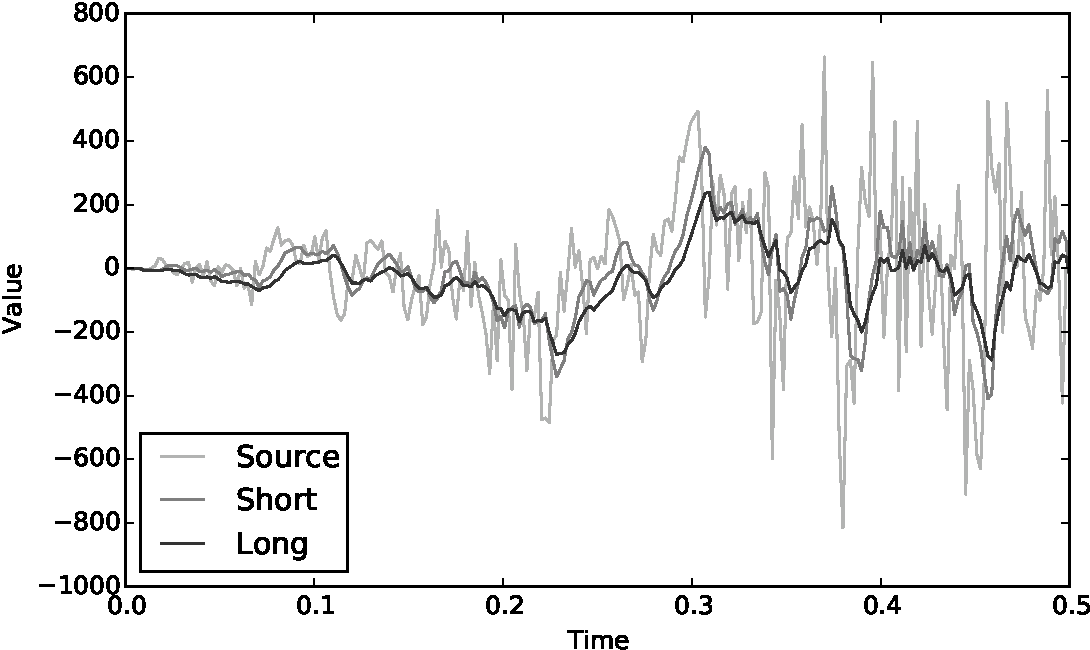
\includegraphics[width=.25\textwidth]{figures/ewma-plot.pdf}};
      }
      ]

      
      \node[proc style] (gen) {Data \\ Generator};
      \node[proc style, right=2cm of gen] (long) {Short Decay};
      \node[proc style, below=0.5cm of long] (short) {Long Decay};
      \node[proc style, below right=0cm and 1.5cm of long] (merge) {Merger};

      \node[proc style, below=0.5cm of gen] (sink) {Plotter};

      \pic[local bounding box=plot, above left=0cm and 2cm of sink] {plot};
      
      \draw[-{Latex[scale=1.6]}] (gen) edge (long);
      \draw[-{Latex[scale=1.6]}] (gen) edge (short);
      \draw[-{Latex[scale=1.6]}] (long) edge (merge);
      \draw[-{Latex[scale=1.6]}] (short) edge (merge);
      \draw[-{Latex[scale=1.6]}] (sink) edge (plot);

      % \draw[-{Latex[scale=1.6]}] (gen) edge (collector);

      \draw[-{Latex[scale=1.6]}] (merge) edge [bend left=50] (sink);
      
      \begin{scope}[on background layer]
        \node[draw=scopeborder,fill=scopebg,inner sep=10pt,rounded corners=10pt,anchor=north west,fit=(long)(short)(merge),label={above}:SMEIL] (SMEIL) {};
        \node[draw=scopeborder,fill=scopebg,inner sep=10pt,rounded corners=10pt,anchor=north west,fit=(gen)(sink),label={above}:PySME] (pysme) {};
      \end{scope}
    \end{tikzpicture}
  }
  \caption{The network of simpletrader.}
  \label{fig:simpletrade}
\end{figure}
We revisit an example from~\cite{asheim2016vhdl}. In high-frequency trading, a
split-second decision needs to be made whether to buy, or sell, a
stock. Reducing latency is paramount as you need to make transactions as fast as
possible. This problem is, therefore, an interesting target for custom hardware
as the intractable latencies induced by general-purpose hardware and
software-implemented decision-making logic are avoided. The real-time value of a
stock is passed through two calculator processes. Both calculate the exponential
moving average of a stock, one using long decay and the other using short
decay. The trading decision is based on detecting when the two averages
cross.~\cite{kablan2012use}

The network is shown in \Cref{fig:simpletrade} and the SMEIL source in
\Cref{fig:tradesrc}. The results of the two calculator processes described above
is passed through the merge process which combines the long and short averages
into a single bus. The core of the trader is written in SMEIL, while the
processes providing input stimuli and data collections is written in Python as a
PySME model. The input data is generated using a Brownian
bridge~\cite{glasserman2003monte} which is a stochastic process commonly used as
a realistic model for simulating stock price developments. The results are
collected and visualized in a graph for easy verification.

In an actual trading chip, the data generator is replaced with actual stock
prices arriving through a network interface and the plot is replaced by market
transactions. Both the testing and verification processes leverage existing
Python libraries. The Brownian bridge generator is implemented using NumPy while
the plot is made using matplotlib. Implementing these test processes in VHDL
would be a massive undertaking, with Python, it is quite simple.

\begin{widefigure}
  \begin{smeilcode2}
sync proc calc (in data, const decay)
  bus result {
    val: int;
    valid: bool;
  };
  var prev: int;

{
  if (data.valid) {
    result.valid = true;
    prev = (data.val >> decay) +
      (prev >> decay) *
      ((1 << decay) - 1);
    result.val = prev;
  } elif (!data.valid) {
    result.val = prev;
  } else {
    result.valid = false;
  }
}

sync proc merge (in long,
                 in short, out res) {
  if (long.valid && short.valid) {
    res.valid = true;
    res.long = long.val;
    res.short = short.val;
  } else {
    res.valid = false;
  }
}

network ewma () {
  const decays: [2]uint = [2, 3];

  exposed bus stream {
    val: int;
    valid: bool;
  };

  exposed bus output {
    short: int;
    long: int;
    valid: bool;
  };

  instance short of calc 
      (data: stream, decay: decays[0]);
  instance long of calc
      (data: stream, decay: decays[1]);
  instance _ of merge
      (long: long.result,
       short: short.result,
       res: output);
}
\end{smeilcode2}
\caption{SMEIL source code for the trader core.}
\label{fig:tradesrc}

\end{widefigure}

\section{MD5 bruteforcer}
\begin{figure}%[tb]
  \centering
  \resizebox{.6\linewidth}{!}{
    \begin{tikzpicture}[font=\small,
      rep style/.style={rectangle,draw=black,text width=1.5cm,minimum
        size=1.5cm,align=center},
      proc style/.style={ellipse,draw=black,align=center,text
        width=1.5cm,minimum size=1.5cm,align=center},
      file style/.style={ellipse,draw=none,align=center,text
        width=1.5cm,minimum size=0.5cm,align=center}
      ]

      \node[proc style] (gen) {Input\\Generator};
      \node[proc style, right=1cm of gen] (calc) {MD5 Hasher};
      \node[proc style, right=1cm of calc] (verify) {Hash\\Verifier};

      \draw[-{Latex[scale=1.6]}] (gen) edge  (calc);
      \draw[-{Latex[scale=1.6]}] (calc) edge  (verify);

    \end{tikzpicture}}
  \caption{Structure of the MD5 bruteforcer network.}
  \label{fig:md5net}
\end{figure}

This example is a simplification of a bruteforcer of MD5-hashes developed to
showcase the performance of FPGAs in comparison with CPUs and GPGPUs for a
trivially parallelizable problem: Bruteforcing an MD5
hash~\cite{johnsen2018md5}. The layout of the network is shown in
\Cref{fig:md5net}. The generator iteratively emits all combinations of 8 ASCII
printable characters as a string. This string is then passed to the hasher,
calculating the MD5 sum of the string. In the verifier, the calculated hash is
compared to a pre-calculated hash of the input string that we wish to find. The
predictiveness of the input generator means that we can ensure that the search
terminates quickly by choosing a target string close to the starting
string. Hence, short runs can be chosen for testing and long runs for
benchmarking.

A complete implementation of this example exists for several targets: CPUs
parallelized with OpenMP, OpenCL for GPGPUs, Xilinx HLS and finally C\# SME.
Both the two latter implementations synthesizes and runs on FPGAs. A comparison
of these implementations showed that while GPUs were superior in raw
performance, the performance-per-watt ratio favored FPGAs by more than an order
of magnitude. Furthermore, the SME version is significantly more efficient than
the Vivado HLS implementation, which relies on the concurrency inference
discussed in the introduction.

This example mainly serves to show an SMEIL implementation of an SME model which
has been synthesized to an FPGA. It also showcases an implementation of a
non-trivial algorithm (MD5) in SMEIL. In particular, the MD5 algorithm relies
heavily on bit-shifting of 32-bit unsigned integers. Therefore, it depends on
the correctness of the integer overflow emulation of the \libsme{} simulator in
order to produce the expected result. The shortened source code of the SMEIL
process for calculating and MD5 hash is shown in \Cref{fig:smeilhash}. The
process receives the string that should be hashed through the bus passed as its
{\ttfamily input} parameter. The calculated hash is then sent on the {\ttfamily
  hashes} bus which is read by the verification process.
% Also note the close
% resemblance of the SMEIL implementation of the algorithm to an eq

\begin{widefigure}

\begin{smeilcode2}
proc md5(in input)
  bus hashes {
    h0: u32;
    h1: u32;
    h2: u32;
    h3: u32;

    w0: u32;
    w1: u32;
  };

  const r: [64]uint = [
    [...]
    6, 10, 15, 21, 6, 10]

  const kk: [64]uint = [
    0xd76aa478, 0xe8c7b756
    [..]
    0xf7537e82, 0xbd3af235
    ];

// Variable declarations omitted

{
  h0 = 0x67452301;
  // [..]

  w[0] = input.w0;
  w[1] = input.w1;
  w[2] = 128;
  w[14] = 64;

  a = h0;
  b = h1;
  c = h2;
  d = h3;

for i = 0 to 63 {
  if (i < 16) {
    f = (b & c) | ((~b) & d);
    g = i;
   // [..]
  } else {
    f = c ^ (b | (~d));
    g = (7 * i) % 16;
  }

  tmp = d;
  d = c;
  c = b;
  x = a + f + kk[i] + w[g];
  c2 = r[i];
  b = b + (((x) << (c2)) |
      ((x) >> (32 - (c2))));
  a = tmp;
}

h0 = h0 + a;
// [..]
h3 = h3 + d;

hashes.h0 = h0;
// [..]
hashes.h3 = h3;

hashes.w0 = w[0];
hashes.w1 = w[1];
}

\end{smeilcode2}
  \caption{SMEIL source code for the MD5 hashing process.}
  \label{fig:smeilhash}

\end{widefigure}

\section{Performance}
The simulation performance of a hardware design tool is not essential as it does
not have an impact on the resulting implementation. Nevertheless, a slow
simulator can waste valuable developer time by inducing a long
develop-compile-test cycle.

The current implementation of SMEIL is not written with performance in mind and
leaves a lot of performance-related low-hanging fruits unpicked. Indeed, its
naïve interpreter makes repeated traversals of the SMEIL AST and the interface
between PySME and \libsme{} relies on the very general and inefficient
\textsc{libffi} library.
% Lastly, Python itself is not cherished for its
% performance. It is therefore noteworthy that it still exceeds the performance of
% the VHDL simulator GHDL,
Lastly, while Python itself is not cherished for its performance, it should be
noted that \libsme{} still exceeds the performance of the VHDL simulator, GHDL, 
which generates native code before simulating. The VHDL
simulator of Xilinx Vivado, fails to complete the simulation due to memory
exhaustion.

Simulating 352,686 cycles of the ColorBin (\Cref{sec:colorbin}) network on an
Intel Core i7 6700HQ CPU at 2.60GHz, requires 47 seconds using GHDL but only 30
seconds using \libsme. Based on the benchmarks shown in \cite{skovhede2017c++},
\libsme{} achieves only slightly lower performance than C\# SME in this
particular test.


%%% Local Variables:
%%% mode: latex
%%% TeX-master: "../master"
%%% TeX-command-extra-options: "-enable-write18"
%%% End:
